
\section{Opérations sur les durées}


%%%%%%%

\begin{methode*1}[Conversion en minutes ou en secondes]

\begin{exemple*1}

\begin{enumerate}
\item Combien y a-t-il de minutes dans 5 h 27 min ?

\begin{tabular}{ll} 
\textcolor{bleu}{\textbf{5 h}} $=$ \textcolor{bleu}{\textbf{5}} $\times$ 60 min $=$ \textcolor{bleu}{\textbf{300 min}}  & $\rightarrow$ Convertir les heures en minutes. \\
\textcolor{bleu}{\textbf{5 h}} \textcolor{vert}{\textbf{27 min}} $=$ \textcolor{bleu}{\textbf{300 min}} $+$ \textcolor{vert}{\textbf{27 min}} $=$ 327 min & $\rightarrow$ Terminer le calcul.\\
%\phantom{2 h 47 min 53 s $=$ 7\,200 s $+$ 2\,820 s $+$ 53} & \\ % phantom pour alignement avec tableau ci-dessous
\end{tabular} 

\vspace{2em}\item Combien y a-t-il de secondes dans 2 h 47 min 53 s ?

\begin{tabular}{ll} 
\textcolor{bleu}{\textbf{2 h}} $=$ \textcolor{bleu}{\textbf{2}} $\times$ 3\,600 s $=$ \textcolor{bleu}{\textbf{7\,200 s}} & $\rightarrow$ Convertir les heures en secondes. \\
\textcolor{vert}{\textbf{47 min}} $=$ \textcolor{vert}{\textbf{47}} $\times$ 60 s $=$ \textcolor{vert}{\textbf{2\,820}} s & $\rightarrow$ Convertir les minutes en secondes. \\
\textcolor{bleu}{\textbf{2 h}} \textcolor{vert}{\textbf{47 min}} 53 s $=$ \textcolor{bleu}{\textbf{7\,200 s}} $+$ \textcolor{vert}{\textbf{2\,820}} s $+$ 53 s  \\
\phantom{2 h 47 min 53 si}$=$ 10\,073 s & $\rightarrow$ Terminer le calcul. \\
\end{tabular}

\end{enumerate}
 
\end{exemple*1}

\exercice

Combien y a-t-il de secondes dans 1 h 52 min 27 s ? Combien y a-t-il de minutes dans un jour ? Dans un an ? Combien y a-t-il de secondes dans un jour ? Dans un an ?

\end{methode*1}



%%%%%%%


\begin{methode*1}[Conversion en heures, minutes et secondes]

\begin{exemple*1}
Combien y a-t-il d'heures, minutes et secondes dans 41\,000 s ? \\[1em]
\begin{minipage}[t]{.46\textwidth}
On convertit les secondes en minutes et secondes en posant la division de 41\,000 par 60 :

\begin{center}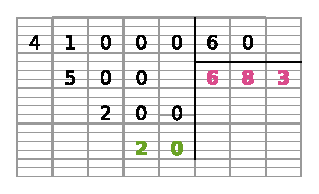
\includegraphics[width=4.6cm]{41000div60} \end{center}

On a donc 41\,000 s $=$ \textcolor{rose}{\textbf{683 min}} \textcolor{vert}{\textbf{20 s}}.
\end{minipage}\hfill%
\begin{minipage}[t]{.46\textwidth}
On convertit alors les minutes en heures et minutes en effectuant la division euclidienne de 683 par 60 :

\begin{center}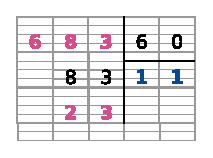
\includegraphics[width=2.9cm]{683div60} \end{center}
On a donc 41\,000 s $=$ \textcolor{bleu}{\textbf{11 h}} \textcolor{rose}{\textbf{23 min}} \textcolor{vert}{\textbf{20 s}}.
\end{minipage}


\end{exemple*1}

\exercice

Combien y a-t-il d'heures, minutes et secondes dans 1\,000\,000 s ?

\end{methode*1}

%%%%%%%%%%%%

\begin{methode*1}[Addition de durées]

\begin{exemple*1}
Un match dure 3 h 38 min et le suivant dure 2 h 49 min. Quelle est la durée totale de ces deux matchs ? \\[1em]
\begin{minipage}[t]{.4\textwidth}
On pose l'addition suivante :\\[0.2em]

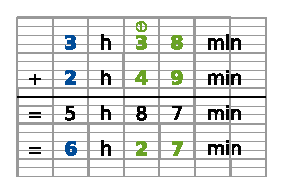
\includegraphics[width=\linewidth]{grille3h38}
\end{minipage}\hfill%
\begin{minipage}[t]{.58\textwidth}
On effectue deux additions indépendantes : 
\textcolor{vert}{\textbf{les minutes entre elles}} et \textcolor{bleu}{\textbf{les heures entre elles}}.\\[0.75em]
Mais le nombre de minutes obtenu est supérieur à 59. 
On va donc le convertir en heures et minutes sachant que 60 min $=$ 1 h. \\[0.75em]
La durée totale de ces deux matchs est donc de \textcolor{rose}{\textbf{6 h 27 min}}.
\end{minipage}

\end{exemple*1}

\exercice

Calcule : 3 h 05 min 13 s $+$ 56 min 48 s et 1 h 46 min $+$ 2 h 37 min.

\end{methode*1}

%%%%%%%%%%%%

\begin{methode*1}[Soustraction de durées]

\begin{exemple*1}
Un film débute à 15 h 27 et finit à 18 h 14. Quelle est la durée de ce film ? \\[1em]

\begin{minipage}[t]{.4\textwidth}
On pose la soustraction suivante :\\[0.2em]

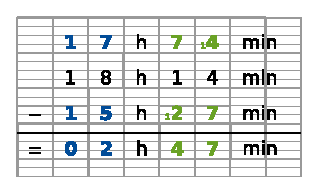
\includegraphics[width=\linewidth]{grille17h74}
\end{minipage}\hfill%
\begin{minipage}[t]{.58\textwidth}
On effectue deux soustractions indépendantes : 
\textcolor{vert}{\textbf{les minutes entre elles}} et \textcolor{bleu}{\textbf{les heures entre elles}}.\\[0.75em]
Mais on ne peut pas enlever 27 à 14. 
On va donc convertir 1 des 18 heures en 60 min. \\[0.75em]
Ce film dure donc \textcolor{rose}{\textbf{2 h 47 min}}.
\end{minipage}

\end{exemple*1}

\exercice

Calcule : 1 h 35 min 29 s $-$ 46 min 37 s et 9 min 16 s $-$ 7 min 55 s.

%\correction

\end{methode*1}
